\documentclass[12pt]{article}
\usepackage{geometry}
\usepackage[spanish]{babel}
\usepackage[utf8]{inputenc}
\usepackage{tocloft}
\usepackage{graphicx}
\usepackage{ragged2e}
\usepackage{natbib}
\usepackage{amsmath}
\usepackage{amsfonts}
\renewcommand{\thesection}{\arabic{section}}
\geometry{
    left=1in,
    right=1in,
    top=1in,
    bottom=1in
}
\linespread{1.5}

\usepackage[colorlinks=true, allcolors=blue]{hyperref}
\hypersetup{
    colorlinks=true,% make the links colored
}
\usepackage{appendix}




\begin{document}   


\begin{titlepage}
    \centering
    \vspace*{2cm}
    
\includegraphics[width=1\textwidth]{logo.png} 
    
    \vspace{2cm}
    {\scshape\LARGE Maestría en Economía} \\
    
    \vspace{0.5cm}
    {\huge\bfseries
    Trabajo Práctico\par}
    \vspace{2cm}
    {\Large\itshape Coloma Conte-Grand, Carolina} \\
    
    {\Large\itshape Condori, Brayan Alexis} \\
    
    {\Large\itshape Deniard, Agustín}
    \vfill
    {\large Profesor: Javier Alejo} \\
    {\large Materia: Regresiones por Cuantiles}

    \vfill

    {\large \today\par}
\end{titlepage}

\justify 

\section*{Ejercicio 1}

\section*{Ejercicio 2}

\section*{Ejercicio 3}

Realizamos un test para estudiar si el efecto parcial de los años de educación sobre el salario es el mismo para los cuantiles condicionales 0.05 y 0.95. Encontramos que el p-valor asociado es de 0,0452, lo cual resulta significativo a 0,05 y nos permite rechazar para este nivel la hipótesis nula de que el efecto parcial de la educación sobre el salario es el mismo en ambos cuantiles.

A su vez, realizamos un test bajo la hipótesis nula de que los coeficientes del modelo (a excepción de la ordenada al origen) no difieren entre cuantiles condicionales. Encontramos que el p-valor asociado es casi nulo, por lo que podemos rechazar la hipótesis nula para un nivel de 0,0001. 

Este test es útil para estudiar la relevancia del modelo ya que muestra si existe o no información adicional proveniente de las regresiones por cuantiles. Si la hipótesis nula no fuera rechazada, esto implicaría que los efectos parciales son iguales sin importar el cuantil, por lo que no habría diferencia entre la información proporcionada por una estimación cuantílica y la obtenida en una regresión por MCO.

\section*{Ejercicio 4}

Graficamos los coeficientes de la regresión en función a los cuantiles $\tau$ estimados. Encontramos que en general todos difieren respecto de la estimación de OLS, aunque esta recta suele encontrarse contenida en la mayoría de los intervalos de confianza estimados por bootstrap. 

\begin{figure}
	\caption{Coeficientes de la regresión respecto al cuantil $\tau$}
	\centering
	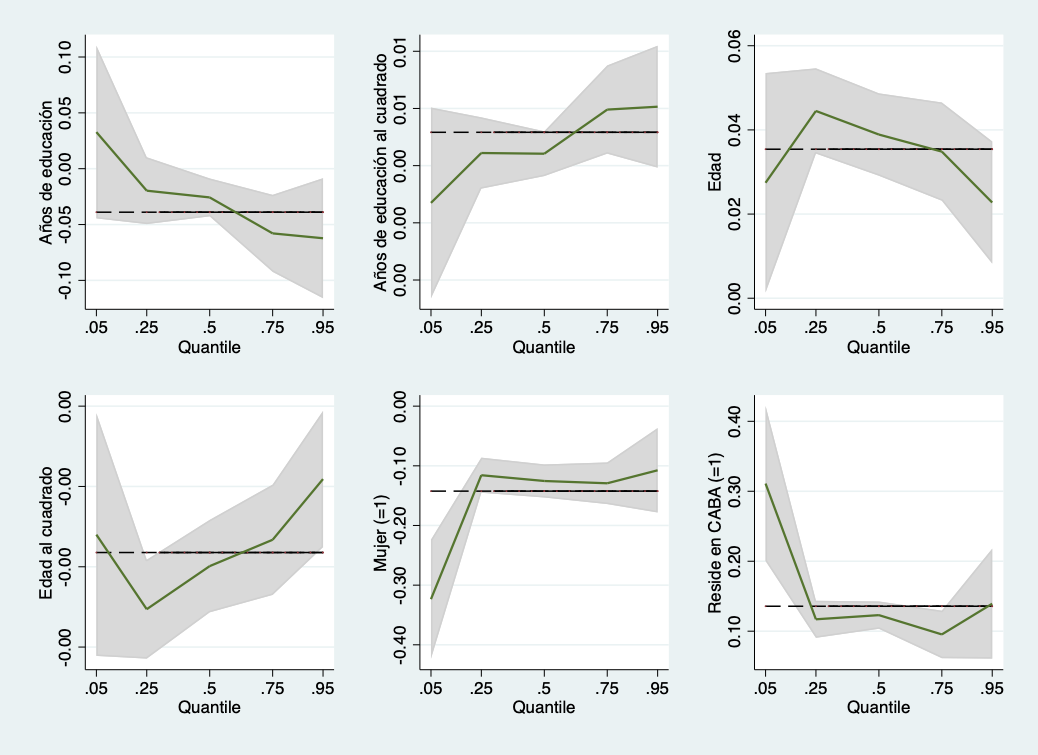
\includegraphics[width=0.8\linewidth]{4.png}
\end{figure}

El método de regresiones por cuantiles es considera uno semiparamétrico. Tiene un componente paramétrico ya que modela a los cuantiles condicionales de la variable dependiente suponiendo una estructura lineal:
\[
Q_y(\tau | X ) = X \beta(\tau)
\]
A su vez, tiene un componente no paramétrico en que no asume una distribución específica para los errores estándares y estima los cuantiles condicionales a partir de la forma de los datos. Por esto se dice que es un método \textit{distribution free}.

\section*{Ejercicio 5}

\end{document}